\documentclass[a4paper]{article}

\usepackage{graphicx}
\usepackage{amsmath,amssymb}
\usepackage{minted}
\usepackage{multirow}
\usepackage{float}
\usepackage{todonotes}
\usepackage{forest}
\usepackage{xstring}
\usepackage{xcolor}
\usepackage[most]{tcolorbox}
\usepackage{xparse}
\usepackage{natbib}

\usetikzlibrary{graphs,graphdrawing}
\usegdlibrary{layered}

% for external graphviz
\input{/home/donkarlo/Dropbox/repo/nd_ai_project/src/nd_ai/knoweldge_representation/language/formal/computer/programming/tex/latex/code_clips/external_graphviz.tex}

% for tags
\input{/home/donkarlo/Dropbox/repo/nd_ai_project/src/nd_ai/knoweldge_representation/language/formal/computer/programming/tex/latex/parts/control_sequence/kind/semtag/semtag.tex}

% for links
\input{/home/donkarlo/Dropbox/repo/nd_ai_project/src/nd_ai/knoweldge_representation/language/formal/computer/programming/tex/latex/code_clips/seehere.tex}

\title{Optical Satellite Imagery}
\date{}
\author{Mohammad Rahmani}

\begin{document}
    \maketitle
    
    
    \section{Optical Satellite Imagery}
        Optical satellite imagery provides repeated, wide-area observations using several spectral bands and consistent acquisition procedures.
        Sentinel-2 is especially useful for regional land-cover analysis, vegetation indices, temporal change detection, and identifying large roof or solar-panel patterns.
        Its freely available global coverage makes it attractive when the same processing pipeline must be scaled beyond one city.
        The main limitation for individual-roof extraction is spatial resolution: a ten-metre pixel can contain several roofs, streets, trees, and shadows at the same time.
        Sentinel data can be searched and downloaded through the Copernicus Data Space Ecosystem \seeherefooter{https://dataspace.copernicus.eu/} and its browser \seeherefooter{https://browser.dataspace.copernicus.eu/}.
        
        \begin{figure}[H]
            \centering
            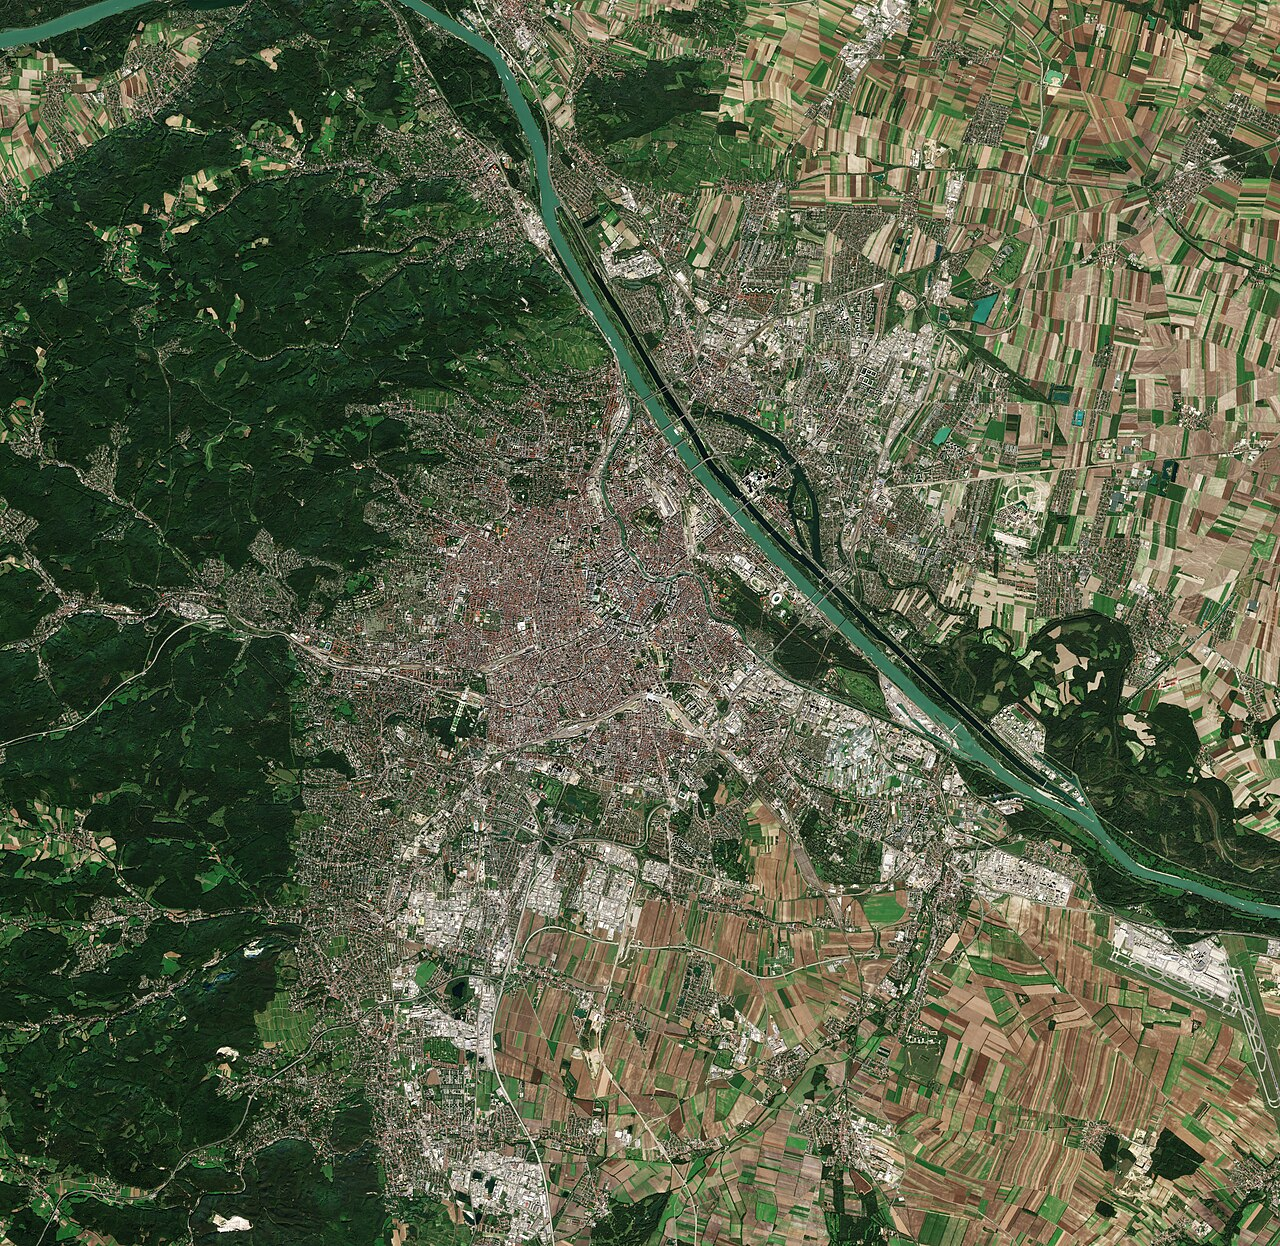
\includegraphics[width=0.58\textwidth]{images/optical_satellite_imagery_example.jpg}
            \caption{Sentinel-2 true-colour image of Vienna, illustrating broad coverage but lower building-level detail.}
        \end{figure}
        \noindent\small Image source and attribution information: \seeherefooter{https://commons.wikimedia.org/w/index.php?oldid=1228010035}.\normalsize

%    \bibliographystyle{plainnat}
%    \bibliography{/home/donkarlo/Dropbox/repo/nd_shared_research/bibliography/bibliography.bib}
\end{document}
